\section{Polarisation Spectroscopy}\label{chapter:pol_spec}

{\color{red}More discussion/intro to pol spec.

Lonely orphans from another section:

Pol Spec developments

It has been shown previously that \gls*{ps} can be used to reduce the linewidth of a distributed feedback diode from \unit[2]{MHz} to \unit[20]{kHz}~\cite{torii_laser-phase_2012} and of \glspl*{ecdl} to \unit[65]{kHz}
~\cite{yoshikawa_frequency_2003}.

Balanced polarimeter.\cite{pearman_polarization_2002,yoshikawa_frequency_2003}

Bi-polarisation spectroscopy.\cite{tiwari_laser_2006}

}

\subsection{Basic Theory}\label{section:pol_spec_theory}

In \gls{ps} a circularly polarised pump beam from a monochromatic laser, with frequency close to an atomic resonance, induces frequency-dependent circular birefringence in a magnetically-shielded atomic gas sample.
A linearly polarised beam from the same source is used to measure the birefringence, monitored with a balanced polarimeter consisting of a half-wave phase retarder, \gls{pbs} and two detectors.
This is shown in Figure \ref{figure:pol_spec_schematic}.

\begin{figure}
\centering
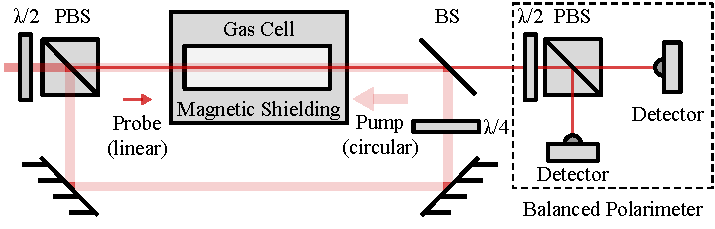
\includegraphics[width=\linewidth]{part1/Figs/PolSpecSchematic.pdf}
\caption{A schematic of \gls{ps} with a balanced polarimeter.
The power balance between the probe and the pump beam is controlled with the left-most $\lambda/2$ phase retarder and \gls{pbs}.
The $\lambda/4$ retarder is adjusted to produce a circularly polarised pump beam.
The non-polarising beamsplitter (BS) is used to counter-propagate the pump beam through the atomic sample without altering the polarisation of the circular pump or linear probe.
The final $\lambda/2$ retarder, \gls{pbs} and the detectors form the balanced polarimeter that monitors the polarisation rotation of the probe.}
\label{figure:pol_spec_schematic}
\end{figure}

The circularly polarised pump beam induces circular birefringence in the atomic sample by partially optically pumping the sample into one of the extreme hyperfine sublevels, $m_F=\pm F$, where $m_F$ labels the hyperfine sublevel and $F$ labels {\color{red}some quantum thingy.}
This partial optical pumping, referred to here as the anisotropy of the medium, results in unequal absorption coefficients for each circular polarisation.
The linearly polarised probe beam can be decomposed into two equal and oppositely circularly polarised components which undergo different absorption due to the anisotropy, such that when recombined after passing through the atomic sample the probe beam becomes elliptically polarised with an angle different to that of the original linear polarisation.
This process is depicted in Figure \ref{figure:pol_spec_explanation}.

\begin{figure}
\centering
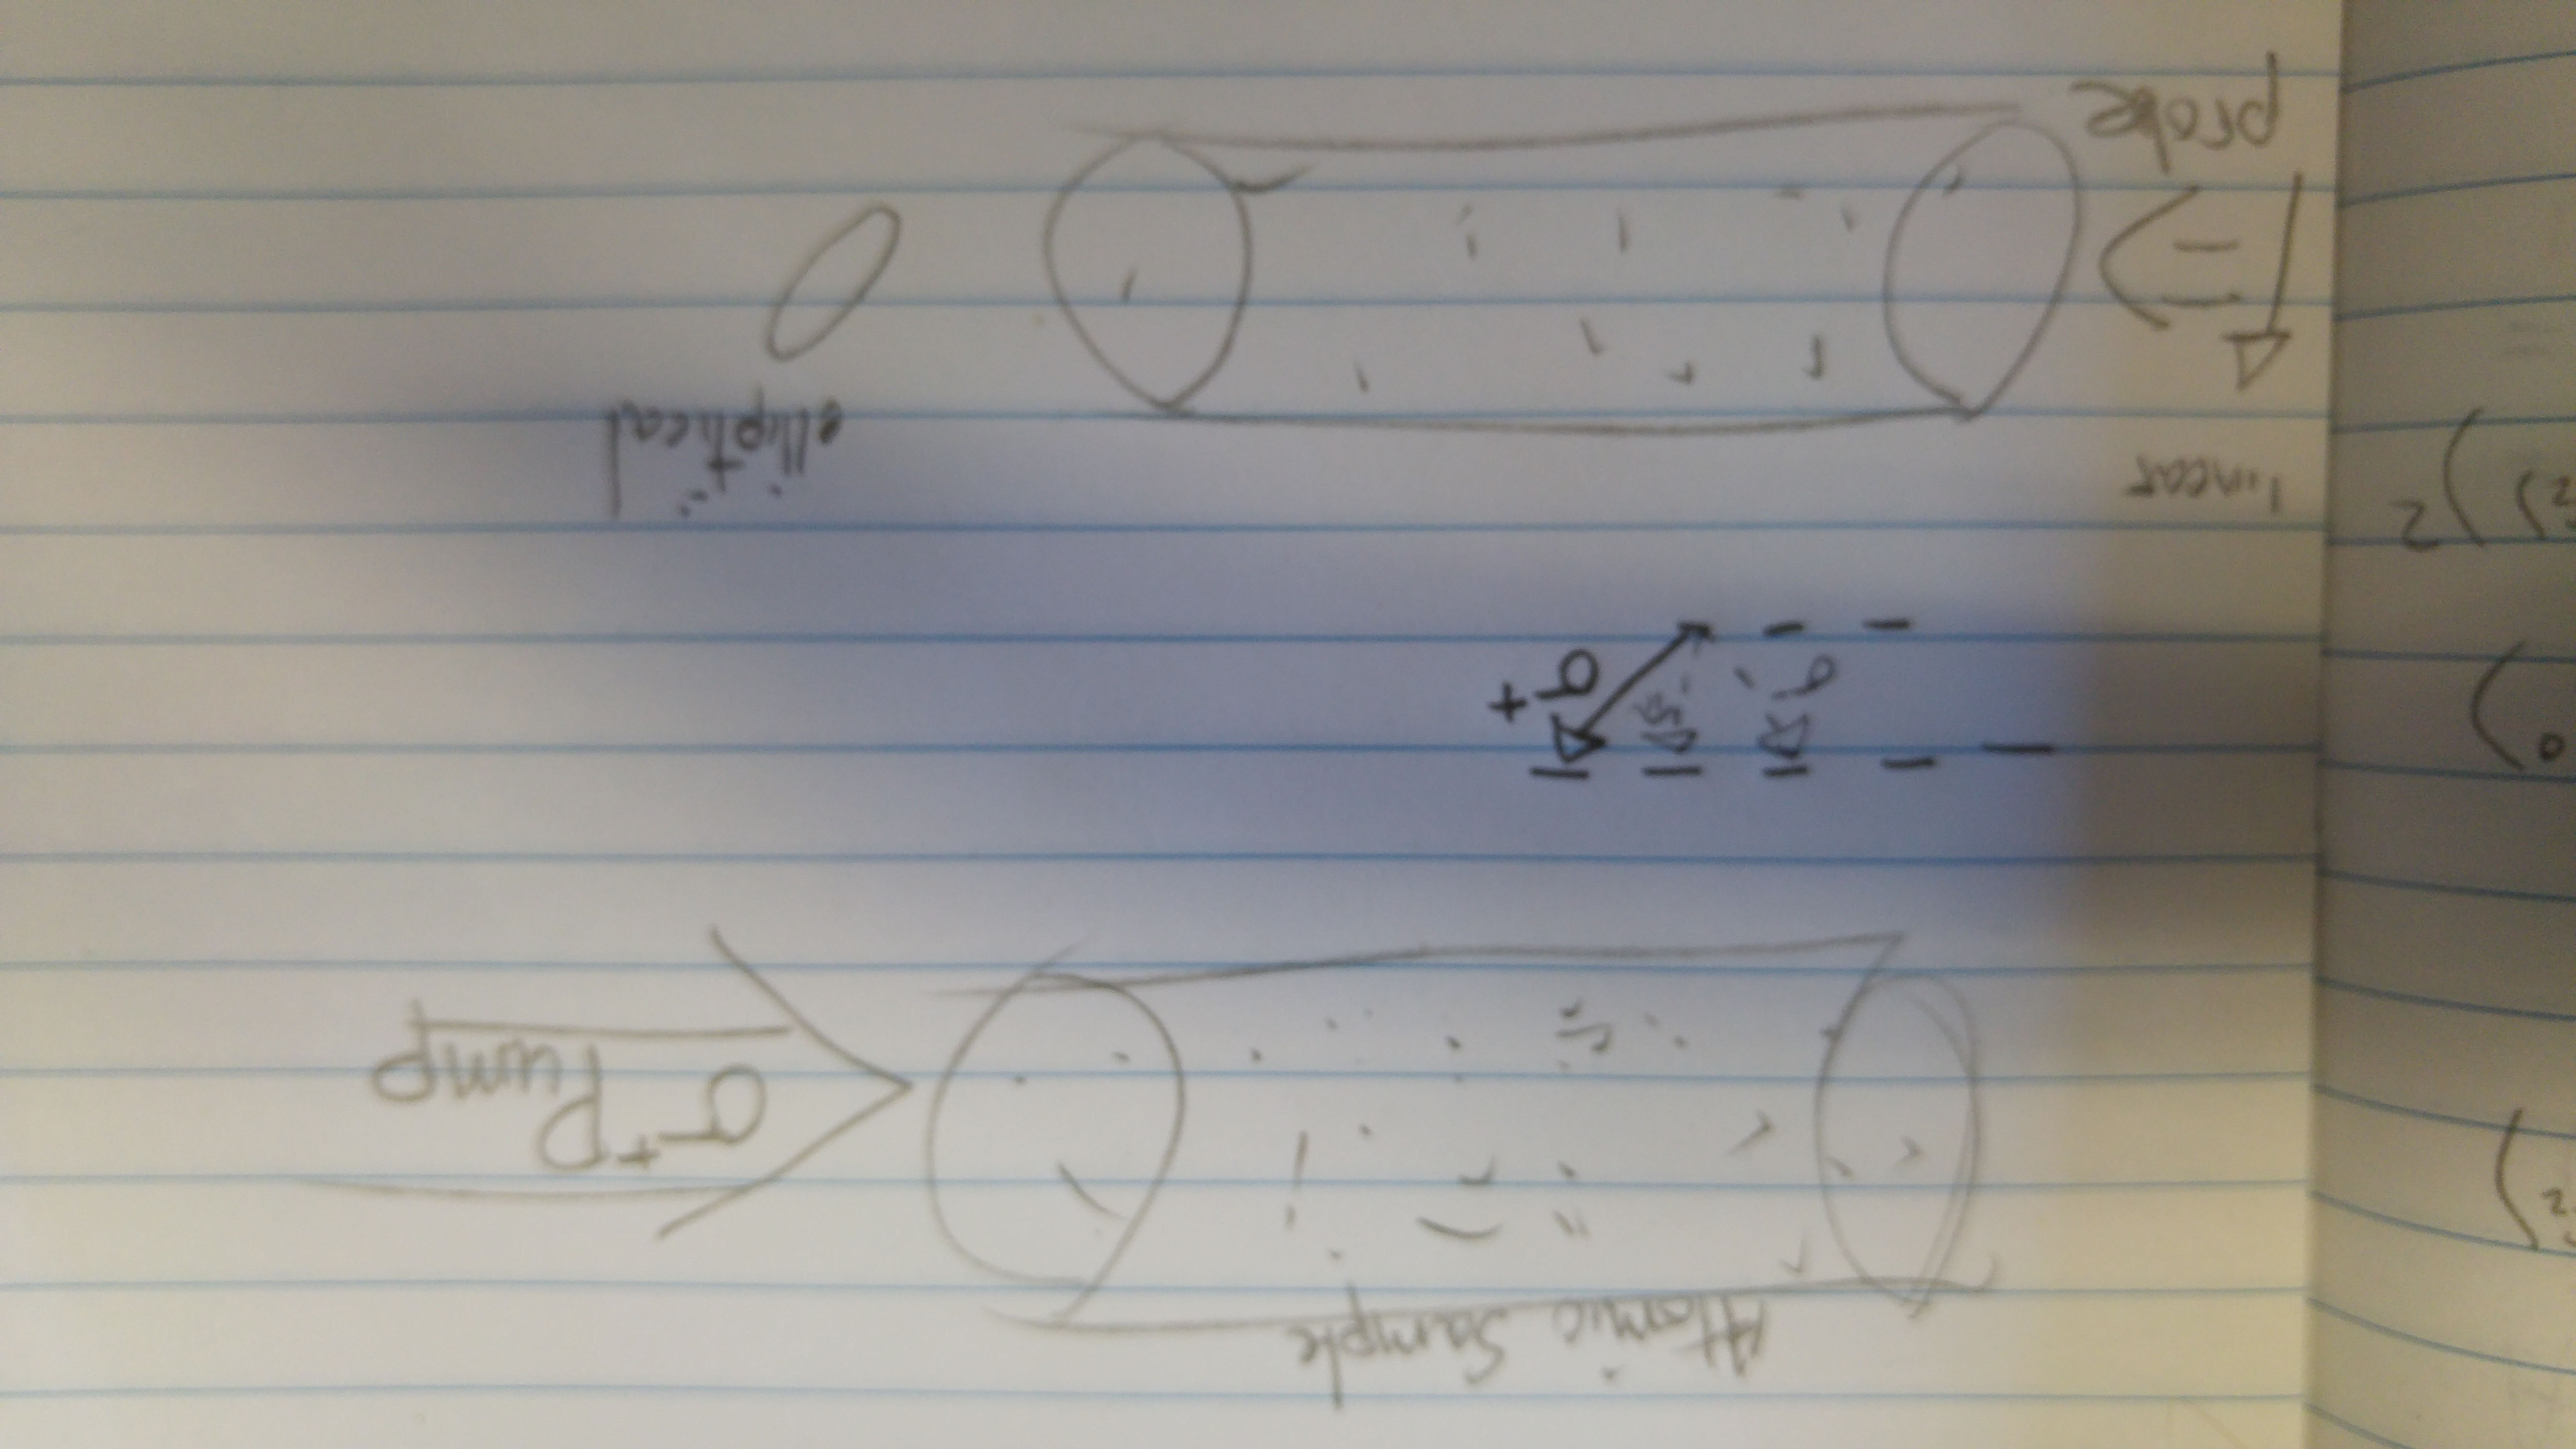
\includegraphics[width=\linewidth,angle=180]{part1/Figs/pol_spec_explanation_placeholder.jpg}
\caption{A conceptual figure for explaining the basics of pol spec.}
\label{figure:pol_spec_explanation}
\end{figure}

Consider the electric field of the probe beam before it enters the atomic sample at an angle $\phi$ to the $x$ axis:
\begin{equation}
\vec{E}=E_0\big(\cos{\phi}\,\hat{x}+\sin{\phi}\,\hat{y}\big)
\end{equation}
which can be expressed in terms of the circularly polarised basis vectors:
\begin{equation}
\vec{E} = \frac{E_0}{2}e^{-i\phi}(\hat{x}+i\hat{y}) + \frac{E_0}{2}e^{+i\phi}(\hat{x}-i\hat{y})
\end{equation}

After propagating through an atomic sample of length $L$ with refractive indices for the circular polarisation components of $n_\pm$, $\vec{E}$ and absorption coefficients of $\alpha_\pm$ the electric field becomes
\begin{align}
\vec{E} = &\frac{E_0}{2}e^{-i\phi}(\hat{x}+i\hat{y})\,\exp\left[\frac{i\omega n_+ L}{c} - \frac{\alpha_+ L}{2}\right] +\notag\\
&\frac{E_0}{2}e^{+i\phi}(\hat{x}-i\hat{y})\,\exp\left[\frac{i\omega n_- L}{c} - \frac{\alpha_- L}{2}\right]\label{equation:elliptically_polarised}
\end{align}

Equation \ref{equation:elliptically_polarised} represents elliptically polarised light with the major axis at an angle of $\theta$ to the $x$-axis, where
\begin{equation}
\theta = \phi + \frac{\pi L (n_+ - n_-)}{\lambda}
\end{equation}
thus the angle by which the probe has rotated is
\begin{equation}
\Phi = \frac{\pi L \Delta n}{\lambda},
\end{equation}
where $\Delta n = n_+ - n_-$.

The electric field after the sample can be approximated to {\color{red}(probably don't need to make this approximation going from 1.3 to 1.7)}
\begin{equation}
\vec{E} = E_0\big(\cos\left[\phi+\Phi\right]\,\hat{x}+\sin\left[\phi+\Phi\right]\,\hat{y}\big).
\end{equation}

The output of the balanced polarimeter is the difference between the intensity {\color{red}(P?)} of light incident on each detector:
\begin{align}
I_{out} = I_x - I_y &= \frac{1}{2}\epsilon_0 c \left(|E_x|^2 - |E_y|^2\right)\notag\\
&= \frac{1}{2}\epsilon_0 c \left(\cos^2\left[\phi+\Phi\right] - \sin^2\left[\phi+\Phi\right]\right)\notag\\
&= \frac{1}{2}\epsilon_0 c \cos\left[2\phi+2\Phi\right]\notag\\
&= I_0 \cos\left[2\phi+2\Phi\right]
\end{align}

The largest spectrum is provided when $\phi=\pi/4$ and since $\Phi$ is small $I_out$ can be approximated to
\begin{equation}
I_{out} = I_0 2\Phi = I_0 \frac{2\pi L \Delta n}{\lambda}
\end{equation}

\subsubsection{Magnetic shielding}

\subsection{Fast Theory}

\subsection{OBEs (timescale of state evolution, step in simulating)}

\subsection{Developments}

\subsubsection{Balanced Polarimeter}
When Wieman and H\"anch~\cite{wieman_doppler-free_1976} originally described \gls{ps} polarisation rotation was monitored with a nearly crossed polariser as shown in Figure \ref{figure:wieman_doppler-free_schematic}.
The polariser is crossed such that only a small proportion of the probe beam passes through them in the absence of the pump.
With the pump inducing anisotropy the rotation of the probe can be detected after the polarisers.

\begin{figure}
\center
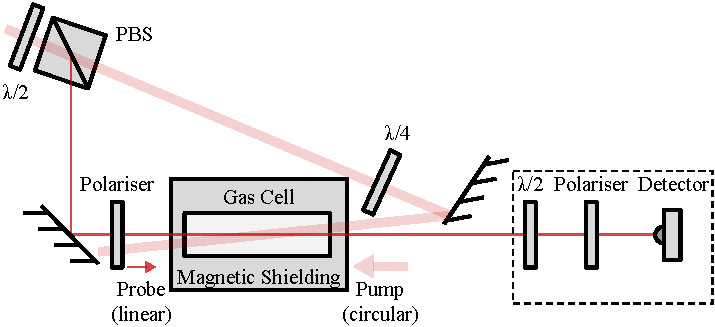
\includegraphics{part1/Figs/PolSpecWieman.pdf}
\caption{Figure stolen from Wieman and H\"anch paper.
Should probably redraw so I'm not plagiarizing.
Or ask how to cite it probably or some such.}
\label{figure:wieman_doppler-free_schematic}
\end{figure}

Pearson et al. proposed the alternative method of using a balanced polarimeter which provides a background-free signal with peak-to-peak height more than an order of magnitude greater than with the crossed polariser method~\cite{pearman_polarization_2002}.

\subsubsection{Beam splitter to co-propagate}

All papers thus far have ``snuck'' the pump beam through the vapour cell.

Figure with ``snucked'' and beam splitter configuration.

The angle of ``snucking'' has implications that there is math for...

Using a NBPS instead means you have an angle of 0.
The beam splitter has no effect on the polarisation as far as I can tell.

Pumped spectroscopy techniques such as \gls{ps} and \gls{sa}... spectral broadening due to angle stuff.

\subsubsection{High bandwidth feedback}


\subsubsection{Lincoln's magic detectors?}

\subsection{Experimental Setup (with details - fibres, calcite, etc.)}

